\documentclass{beamer}                             % presentation
% \documentclass[draft]{beamer}                      % improves compile time
\usepackage[utf8]{inputenc}                        % utf8
\usepackage[T1]{fontenc}                           % fix font encoding
\usepackage[english]{babel}                        % language
\usepackage[autostyle, english=american]{csquotes} % quotes
\usepackage{bm, mathtools}                         % extra math packages
\usepackage{graphicx, subcaption}                  % images
\usepackage{tikz, pgfplots}                        % plots and graphs
\usepackage[style=authoryear-comp]{biblatex}       % bibliography
\usepackage{geometry, hyperref}                    % misc.

\usetikzlibrary{positioning}                       % advanced positioning
\pgfplotsset{compat=newest}                        % version of pgfplots

\graphicspath{{./figures/}}
\addbibresource{cholesky.bib}
\addbibresource{references.bib}

%%% math

% serif font in math mode
\usefonttheme[onlymath]{serif}

\newcommand*{\defeq}{\coloneqq}
\newcommand*{\BigO}{\mathcal{O}}
\newcommand*{\N}{\mathcal{N}}
\newcommand*{\SpSet}{\mathcal{S}}
\newcommand*{\GP}{\mathcal{GP}}
\newcommand*{\Loss}{\mathcal{L}}
\newcommand*{\Order}{\mathcal{I}}
\newcommand*{\Reverse}{\updownarrow}
\newcommand*{\I}{I}
\newcommand*{\J}{J}
\newcommand*{\V}{V}
\newcommand*{\dd}{\, \text{d}}
\renewcommand*{\vec}[1]{\bm{#1}}
\newcommand*{\Id}{\text{Id}}

% Names of variables
% covariance matrix
\newcommand*{\CM}{\Theta}
% precision matrix
\newcommand*{\PM}{Q}
\newcommand*{\mean}{\mu}
\newcommand*{\var}{\sigma^2}
\newcommand*{\std}{\sigma}
% kernel function
\newcommand*{\K}{K}
\newcommand*{\Train}{\text{Tr}}
\newcommand*{\Pred}{\text{Pr}}

% Names of operators
\DeclarePairedDelimiter{\norm}{\lVert}{\rVert}
\DeclarePairedDelimiter{\abs}{\lvert}{\rvert}
\DeclarePairedDelimiter{\card}{\lvert}{\rvert}
\DeclareMathOperator{\diag}{diag}
\let\trace\relax
\DeclareMathOperator{\trace}{trace}
\DeclareMathOperator{\logdet}{logdet}
\DeclareMathOperator{\chol}{chol}
\DeclareMathOperator{\FRO}{FRO}

\DeclareMathOperator*{\argmin}{argmin}
\DeclareMathOperator*{\argmax}{argmax}

\DeclarePairedDelimiterX{\infdivx}[2]{(}{)}{%
  #1\;\delimsize\|\;#2%
}
\newcommand*{\KL}{\mathbb{D}_{\operatorname{KL}}\infdivx}
\DeclareMathOperator{\p}{\pi}
\DeclareMathOperator{\E}{\mathbb{E}}
\DeclareMathOperator{\Var}{\mathbb{V}ar}
\DeclareMathOperator{\Cov}{\mathbb{C}ov}
\DeclareMathOperator{\Corr}{\mathbb{C}orr}
\DeclareMathOperator{\entropy}{\mathbb{H}}
\DeclareMathOperator{\MI}{\mathbb{I}}

%%% colors

\definecolor{lightblue}{HTML}{a1b4c7}
\definecolor{orange}{HTML}{ea8810}
\definecolor{silver}{HTML}{b0aba8}
\definecolor{rust}{HTML}{b8420f}
\definecolor{seagreen}{HTML}{23553c}

\colorlet{lightsilver}{silver!20!white}
\colorlet{darkorange}{orange!85!black}
\colorlet{darksilver}{silver!85!black}
\colorlet{darklightblue}{lightblue!75!black}
\colorlet{darkrust}{rust!85!black}
\colorlet{darkseagreen}{seagreen!85!black}

\colorlet{zeroborder}{darksilver}
\colorlet{zerocolor}{lightsilver}
\colorlet{nnzborder}{darksilver}
\colorlet{nnzcolor}{silver}

\colorlet{colborder}{black}
\colorlet{targetcolor}{orange}
\colorlet{selcolor}{seagreen}
\colorlet{candcolor}{lightblue}

\hypersetup{
  colorlinks=true,
  linkcolor=darkrust,
  citecolor=darkseagreen,
  urlcolor=darksilver
}

\pgfplotsset{compat=newest}
\usepgfplotslibrary{fillbetween}
% make marks not follow the style of lines
\tikzset{every mark/.append style={solid}}
% cache tikz graphics
% \usepgfplotslibrary{external}
% \tikzexternalize
% \tikzsetexternalprefix{external/}

%%% beamer settings

\usetheme{Pittsburgh}
\usecolortheme{dolphin}

% hide navigation buttons
\setbeamertemplate{navigation symbols}{}
% change title color
\setbeamercolor{title}{fg=darklightblue}
\setbeamercolor{frametitle}{fg=darklightblue}
% table of contents
\setbeamertemplate{section in toc}[default]
% change bibliography entry colors
\setbeamercolor{bibliography entry author}{fg=darklightblue}
\setbeamercolor{bibliography entry note}{fg=lightblue}
% customize \item in itemize
\setbeamercolor{structure}{fg=darklightblue}
\setbeamertemplate{itemize item}{}
\setbeamertemplate{enumerate item}[default]
% enumitem doesn't play well with beamer
% \setitemize{label={},itemsep=0.5cm}
% https://tex.stackexchange.com/questions/16793/
\newenvironment{wideitemize}
  {\itemize\setlength{\itemsep}{0.5cm}}
  {\enditemize}

% title page
\title[]{Scalable Gaussian processes for \\ non-ergodic earthquake models}
\subtitle{}
\author[Huan]{Stephen\ Huan}
\institute[Georgia Institute of Technology]
{
  % Georgia Institute of Technology
  \url{https://cgdct.moe}
}
\date[]{SURF Summer Seminar Day 2023}
\subject{K - Computer Science and Applied and Computational Mathematics}

% https://sfp.caltech.edu/undergraduate-research/summer_requirements/final_presentation

\begin{document}

\frame{\titlepage}

\begin{frame}
\frametitle{Collaborators}
\framesubtitle{}
  \begin{columns}
    \begin{column}{0.26\textwidth}
      \centering
      \begin{figure}[h!]
        \centering
        % https://tex.stackexchange.com/questions/41370
        % latex renders at 72 dpi for "px"
        \includegraphics[
          width=2cm,
          height=2cm,
          trim={33.75px 0 33.75px 0},
          clip,
        ]{figures/people/houman_owhadi.jpg}
      \end{figure}
      Houman Owhadi, \\ Caltech
    \end{column}
    \begin{column}{0.28\textwidth}
      \centering
      \begin{figure}[h!]
        \centering
        \includegraphics[
          width=2cm,
          height=2cm,
          trim={0 40px 0 19px},
          clip,
        ]{figures/people/greg_lavrentiadis.jpg}
      \end{figure}
      Greg Lavrentiadis, \\ Caltech
    \end{column}
    \begin{column}{0.22\textwidth}
      \centering
      \begin{figure}[h!]
        \centering
        \includegraphics[
          width=2cm,
          height=2cm,
        ]{figures/people/yifan_chen.jpg}
      \end{figure}
      Yifan Chen, \\ Caltech
    \end{column}
    \begin{column}{0.22\textwidth}
      \centering
      \begin{figure}[h!]
        \centering
        \includegraphics[
          width=2cm,
          height=2cm,
          trim={0 20px 0 21px},
          clip,
        ]{figures/people/pau_batlle.jpg}
      \end{figure}
      Pau Batlle, \\ Caltech
    \end{column}
  \end{columns}
\end{frame}

\begin{frame}
\frametitle{Collaborators}
\framesubtitle{}
\begin{columns}
  \begin{column}{\textwidth}
    \centering
    \begin{figure}[h!]
      \centering
      \includegraphics[
        width=2cm,
        height=2cm,
        trim={0 0 0 46px},
        clip
      ]{figures/people/florian_schaefer.jpg}
    \end{figure}
    Florian\ Sch{\"a}fer, \\ Gatech
  \end{column}
\end{columns}
\end{frame}

\begin{frame}
\frametitle{Overview}
\framesubtitle{}

\tableofcontents
\end{frame}

\section{Introduction}

\begin{frame}
\frametitle{The problem}
\framesubtitle{}

\begin{wideitemize}
  \item<+-> Non-ergodic ground-motion models [\cite{lavrentiadis2022overview}]
    estimate the probability an earthquake exceeds a fixed intensity
  \item<+-> \emph{Ergodic} refers to assumption of translation invariance
  \item<+-> Gaussian process modeling provides uncertainty quantification
  \item<+-> Seismic hazard at nuclear power plant locations
\end{wideitemize}
\end{frame}

\section{Gaussian process modelling}

\begin{frame}
\frametitle{Gaussian process regression}
\framesubtitle{}

\begin{wideitemize}
  \item<+-> Given dataset \( \mathcal{D} = \{ (\vec{x}_i, y_i)
    \}_{i = 1}^N \), learn residual \( y_i = f(\vec{x}_i) \)
  \item<+-> Gaussian process (GP) modeling
    \( f \sim \GP(\mu(\cdot), \K(\cdot, \cdot)) \)
  \item<+-> Use closed-form posterior predictions
    \begin{align*}
      \E[\vec{y}_\Pred \mid \vec{y}_\Train] &=
        \vec{\mean}_\Pred +
        \CM_{\Pred, \Train} \CM_{\Train, \Train}^{-1}
        (\vec{y}_\Train - \vec{\mean}_\Train) \\
      \Cov[\vec{y}_\Pred \mid \vec{y}_\Train] &=
        \CM_{\Pred, \Pred} -
        \CM_{\Pred, \Train} \CM_{\Train, \Train}^{-1}
        \CM_{\Train, \Pred}
    \end{align*}
    \item<+-> Direct computation scales as \(
      \BigO(N^3) \), limiting data size (\( 10^4 \))
  \end{wideitemize}
\end{frame}

\begin{frame}
\frametitle{Mat{\'e}rn kernel functions}
\framesubtitle{}

\begin{wideitemize}
  \item Mat{\'e}rn family of kernels with
    smoothness \( \nu \) and length scale \( \ell \)
  \item\( \nu = 1/2 \) corresponds to the
    exponential kernel \( \psi^2 \exp(-r/\ell) \)
  \item \( \nu = \infty \) to the squared
    exponential kernel \( \psi^2 \exp(-r^2/(2 \ell^2)) \)
\end{wideitemize}
\begin{figure}[b]
  \centering
  \includegraphics[width=0.45\textwidth]{figures/matern/exp.png}%
  \qquad%
  \includegraphics[width=0.45\textwidth]{figures/matern/sqexp.png}%
\end{figure}
\end{frame}

\begin{frame}
\frametitle{Kernel function}
\framesubtitle{}

\begin{wideitemize}
  \item<+-> Use kernel
    \begin{align*}
      c_1(t_E)
      + c_2(t_S)
      + X_3 c_3 (t_E, t_S)
      + [\Delta R \cdot c_{\text{ca}}(t_C)]
      + \delta W
      + \delta B
    \end{align*}
  where
    \begin{itemize}
      \item \( c_1 \) models earthquake interactions
      \item \( c_2 \) models site (receiver) interactions
      \item \( X_3 \) is the geometric scaling spreading
      \item \( c_3 \) models the interaction between earthquakes and sites
      \item \( \Delta R \) is a cell path distance array
      \item \( c_{\text{ca}} \) models cell-specific path attenuation
      \item \( \delta W \) is a noise nugget
      \item \( \delta B \) is noise shared within the same earthquake event
    \end{itemize}
\end{wideitemize}
\end{frame}

\begin{frame}
\frametitle{Modeling overview}
\framesubtitle{}

\begin{wideitemize}
  \item Pick (parametric) class of kernel functions
  \item Learn hyperparameters (MLE, full Bayesian, kernel flows, \ldots)
  \item Make predictions
\end{wideitemize}
\end{frame}

\begin{frame}
\frametitle{What do we need?}
\framesubtitle{}

\begin{wideitemize}
  \item<+-> (log-)Likelihood, posterior statistics
    \begin{align*}
      -2 \log \eta(\vec{y}) &=
        \logdet(\CM)
        + \vec{y}^{\top} \CM^{-1} \vec{y}
        + N \log(2 \pi) \\
      \E[\vec{y}_\Pred \mid \vec{y}_\Train] &=
        \CM_{\Pred, \Train} \CM_{\Train, \Train}^{-1} \vec{y}_\Train \\
      \Cov[\vec{y}_\Pred \mid \vec{y}_\Train] &=
        \CM_{\Pred, \Pred} -
        \CM_{\Pred, \Train} \CM_{\Train, \Train}^{-1}
        \CM_{\Train, \Pred}
    \end{align*}
  \item<+-> Log determinant, inversion
  \item<+-> Accelerated with \emph{Cholesky factor} \( \CM = L L^{\top} \)
  \item<+-> Seek \emph{sparse} Cholesky
    factor for \emph{dense} covariance matrix
\end{wideitemize}
\end{frame}

\section{Sparse Cholesky factorization}

% \begin{frame}
% \frametitle{Statistical interpretation of s.p.d.\ matrices}
% % \framesubtitle{Covariance or precision?}
%
% \begin{wideitemize}
%   \item<+-> Factor covariance matrix \( \CM \)
%     or precision matrix \( \PM \defeq \CM^{-1} \)?
%     \begin{align*}
%       \CM_{i, i}      &= \Var[y_i] &
%       \PM_{i, i}^{-1} &= \Var[y_i \mid y_{k \neq i}] \\
%       \CM_{i, j} &= \Cov[y_i, y_j] &
%       \frac{-\PM_{i, j}}{\sqrt{\PM_{i, i} \PM_{j, j}}} &=
%         \Corr[y_i, y_j \mid y_{k \neq i, j}]
%     \end{align*}
%   \item<+-> Covariance matrix encodes marginal independence
%   \item<2-> Precision matrix encodes conditional independence
%   \item<+-> Prefer precision matrix to attenuate density
% \end{wideitemize}
% \end{frame}

\begin{frame}
\frametitle{Statistical Cholesky factorization}
% \framesubtitle{Covariance or precision?}

\begin{wideitemize}
  \item<+-> Cholesky factorization \( \Leftrightarrow
    \) iterative conditioning of process
    \begin{align*}
      % observation 1 and observation 2 from phd thesis
      % L &= \chol(\CM) &
      L &= \chol(\CM^{-1}) \\
      % L_{i, j} &=
      %   \frac{\Cov[y_i, y_j \mid y_{k < j}]}
      %  {\sqrt{\Var[y_j      \mid y_{k < j}]}} &
      -\frac{L_{i, j}}{L_{j, j}} &=
        \frac{\Cov[y_i, y_j \mid y_{k > j, k \neq i}]}
             {\Var[y_j      \mid y_{k > j, k \neq i}]}
    \end{align*}
  \item<+-> Conditional (near)-independence \(
    \Leftrightarrow \) (approximate) sparsity
\end{wideitemize}
\end{frame}

\begin{frame}
\frametitle{Screening effect}
\framesubtitle{}

\begin{figure}[t]
  \centering
  \begin{tikzpicture}[baseline]
  \begin{axis}[
    width={0.45\textwidth},
    grid={major},
    scale only axis={true},
    xticklabels=none,
    yticklabels=none,
    zticklabels=none,
    xmin=-1.1, xmax=1.1, ymin=-1.1, ymax=1.1, zmin=-0.1, zmax=1,
  ]
  \addplot3 [only marks, orange, mark size=8]
    table {figures/screening/matern_uncond_points.csv};
  \addplot3 [mesh, lightblue, ultra thick]
    table {figures/screening/matern_uncond.csv};
  \end{axis}
\end{tikzpicture}
%
  \qquad
  \input{figures/screening/cond.tex}
\end{figure}

\begin{wideitemize}
  \item<+-> Conditional on points near a point of interest, \\
    far away points are almost independent [\cite{stein2002screening}]
  \item<+-> Suggests space-covering ordering
    and selecting nearby points % for the sparsity
\end{wideitemize}
\end{frame}

\begin{frame}
\frametitle{Cholesky factorization recipe}
\framesubtitle{}

\begin{wideitemize}
  \item<+-> Implied procedure for computing \( L L^{\top} \approx \CM^{-1} \)
    \begin{enumerate}
      \item Pick an ordering on the rows/columns of \( \CM \)
      \item Select a sparsity pattern lower triangular w.r.t. ordering
      \item Compute entries by minimizing objective over all factors
    \end{enumerate}
\end{wideitemize}
\end{frame}

\begin{frame}
\frametitle{Ordering and sparsity pattern}
\framesubtitle{}

% copied a bit from https://youtu.be/Hdhv-moeR5U?t=968
\begin{wideitemize}
  \item (Reverse) maximin ordering [\cite{guinness2018permutation}]
    selects the next \textcolor{orange}{point \( \vec{x}_i \)}
    with \textcolor{orange}{largest distance \( \ell_i \)} to
    \textcolor{lightblue}{points selected before}
  \item The \( i \)th column selects all points
    within a radius of \textcolor{seagreen}{\( \rho
    \ell_i \)} from \textcolor{orange}{\( \vec{x}_i \)}
\end{wideitemize}

% computer generated
\only<1>{
  \begin{figure}
    \centering
    \input{figures/points_knn/cholesky_factor_01.tex}%
    \qquad
    \input{figures/points_knn/selected_points_01.tex}
  \end{figure}
}
\only<2>{
  \begin{figure}
    \centering
    \input{figures/points_knn/cholesky_factor_02.tex}%
    \qquad
    \begin{tikzpicture}[baseline]
  \begin{axis}[
    % calculated from Cholesky factor, exactly 16 cm x 16 cm
    width={4cm},
    height={4cm},
    axis lines={none},
    % force axis box to have exactly the right dimensions, ignoring labels
    scale only axis=true,
  ]
  % consistent size bounding box
  \draw [white, line width=0] (-0.1, -0.1) -- (-0.1,  1.1);
  \draw [white, line width=0] ( 1.1, -0.1) -- ( 1.1,  1.1);
  \draw [white, line width=0] (-0.1, -0.1) -- (-1.1, -0.1);
  \draw [white, line width=0] (-0.1,  1.1) -- (-1.1,  1.1);
  \draw [seagreen!15, fill, radius=1.9421300888061523] (0.7378377872921602, 0.9562672548360985) circle;
  \draw [seagreen, radius=1.9421300888061523] (0.7378377872921602, 0.9562672548360985) circle;
  \draw [orange!25, fill, radius=0.9710650444030762] (0.7378377872921602, 0.9562672548360985) circle;
  \draw [orange, radius=0.9710650444030762] (0.7378377872921602, 0.9562672548360985) circle;
  \addplot [only marks, mark size=1, silver]    table
    {figures/points_knn/all_points.csv};
  \addplot [only marks, mark size=2, lightblue] table
    {figures/points_knn/candidates_02.csv};
  \addplot [only marks, mark size=4, seagreen]  table
    {figures/points_knn/selected_02.csv};
  \addplot [only marks, mark size=4, orange]    table
    {figures/points_knn/target_02.csv};
  \end{axis}
\end{tikzpicture}

  \end{figure}
}
\only<3>{
  \begin{figure}
    \centering
    \input{figures/points_knn/cholesky_factor_03.tex}%
    \qquad
    \begin{tikzpicture}[baseline]
  \begin{axis}[
    % calculated from Cholesky factor, exactly 16 cm x 16 cm
    width={4cm},
    height={4cm},
    axis lines={none},
    % force axis box to have exactly the right dimensions, ignoring labels
    scale only axis=true,
  ]
  % consistent size bounding box
  \draw [white, line width=0] (-0.1, -0.1) -- (-0.1,  1.1);
  \draw [white, line width=0] ( 1.1, -0.1) -- ( 1.1,  1.1);
  \draw [white, line width=0] (-0.1, -0.1) -- (-1.1, -0.1);
  \draw [white, line width=0] (-0.1,  1.1) -- (-1.1,  1.1);
  \draw [seagreen!15, fill, radius=1.4730958938598633] (0.0014900835088361708, 0.9734602747664127) circle;
  \draw [seagreen, radius=1.4730958938598633] (0.0014900835088361708, 0.9734602747664127) circle;
  \draw [orange!25, fill, radius=0.7365479469299316] (0.0014900835088361708, 0.9734602747664127) circle;
  \draw [orange, radius=0.7365479469299316] (0.0014900835088361708, 0.9734602747664127) circle;
  \addplot [only marks, mark size=1, silver]    table
    {figures/points_knn/all_points.csv};
  \addplot [only marks, mark size=2, lightblue] table
    {figures/points_knn/candidates_03.csv};
  \addplot [only marks, mark size=4, seagreen]  table
    {figures/points_knn/selected_03.csv};
  \addplot [only marks, mark size=4, orange]    table
    {figures/points_knn/target_03.csv};
  \end{axis}
\end{tikzpicture}

  \end{figure}
}
\only<4>{
  \begin{figure}
    \centering
    \input{figures/points_knn/cholesky_factor_04.tex}%
    \qquad
    \begin{tikzpicture}[baseline]
  \begin{axis}[
    % calculated from Cholesky factor, exactly 16 cm x 16 cm
    width={4cm},
    height={4cm},
    axis lines={none},
    % force axis box to have exactly the right dimensions, ignoring labels
    scale only axis=true,
  ]
  % consistent size bounding box
  \draw [white, line width=0] (-0.1, -0.1) -- (-0.1,  1.1);
  \draw [white, line width=0] ( 1.1, -0.1) -- ( 1.1,  1.1);
  \draw [white, line width=0] (-0.1, -0.1) -- (-1.1, -0.1);
  \draw [white, line width=0] (-0.1,  1.1) -- (-1.1,  1.1);
  \draw [seagreen!15, fill, radius=1.3210153579711914] (0.7345771514092145, 0.11367201992140341) circle;
  \draw [seagreen, radius=1.3210153579711914] (0.7345771514092145, 0.11367201992140341) circle;
  \draw [orange!25, fill, radius=0.6605076789855957] (0.7345771514092145, 0.11367201992140341) circle;
  \draw [orange, radius=0.6605076789855957] (0.7345771514092145, 0.11367201992140341) circle;
  \addplot [only marks, mark size=1, silver]    table
    {figures/points_knn/all_points.csv};
  \addplot [only marks, mark size=2, lightblue] table
    {figures/points_knn/candidates_04.csv};
  \addplot [only marks, mark size=4, seagreen]  table
    {figures/points_knn/selected_04.csv};
  \addplot [only marks, mark size=4, orange]    table
    {figures/points_knn/target_04.csv};
  \end{axis}
\end{tikzpicture}

  \end{figure}
}
\only<5>{
  \begin{figure}
    \centering
    \input{figures/points_knn/cholesky_factor_05.tex}%
    \qquad
    \begin{tikzpicture}[baseline]
  \begin{axis}[
    % calculated from Cholesky factor, exactly 16 cm x 16 cm
    width={4cm},
    height={4cm},
    axis lines={none},
    % force axis box to have exactly the right dimensions, ignoring labels
    scale only axis=true,
  ]
  % consistent size bounding box
  \draw [white, line width=0] (-0.1, -0.1) -- (-0.1,  1.1);
  \draw [white, line width=0] ( 1.1, -0.1) -- ( 1.1,  1.1);
  \draw [white, line width=0] (-0.1, -0.1) -- (-1.1, -0.1);
  \draw [white, line width=0] (-0.1,  1.1) -- (-1.1,  1.1);
  \draw [seagreen!15, fill, radius=0.9610095024108887] (0.4306280204141778, 0.5867985714381407) circle;
  \draw [seagreen, radius=0.9610095024108887] (0.4306280204141778, 0.5867985714381407) circle;
  \draw [orange!25, fill, radius=0.48050475120544434] (0.4306280204141778, 0.5867985714381407) circle;
  \draw [orange, radius=0.48050475120544434] (0.4306280204141778, 0.5867985714381407) circle;
  \addplot [only marks, mark size=1, silver]    table
    {figures/points_knn/all_points.csv};
  \addplot [only marks, mark size=2, lightblue] table
    {figures/points_knn/candidates_05.csv};
  \addplot [only marks, mark size=4, seagreen]  table
    {figures/points_knn/selected_05.csv};
  \addplot [only marks, mark size=4, orange]    table
    {figures/points_knn/target_05.csv};
  \end{axis}
\end{tikzpicture}

  \end{figure}
}
\only<6>{
  \begin{figure}
    \centering
    \input{figures/points_knn/cholesky_factor_06.tex}%
    \qquad
    \input{figures/points_knn/selected_points_06.tex}
  \end{figure}
}
\only<7>{
  \begin{figure}
    \centering
    \input{figures/points_knn/cholesky_factor_07.tex}%
    \qquad
    \begin{tikzpicture}[baseline]
  \begin{axis}[
    % calculated from Cholesky factor, exactly 16 cm x 16 cm
    width={4cm},
    height={4cm},
    axis lines={none},
    % force axis box to have exactly the right dimensions, ignoring labels
    scale only axis=true,
  ]
  % consistent size bounding box
  \draw [white, line width=0] (-0.1, -0.1) -- (-0.1,  1.1);
  \draw [white, line width=0] ( 1.1, -0.1) -- ( 1.1,  1.1);
  \draw [white, line width=0] (-0.1, -0.1) -- (-1.1, -0.1);
  \draw [white, line width=0] (-0.1,  1.1) -- (-1.1,  1.1);
  \draw [seagreen!15, fill, radius=0.6468091011047363] (0.3742438334784708, 0.09085271350425783) circle;
  \draw [seagreen, radius=0.6468091011047363] (0.3742438334784708, 0.09085271350425783) circle;
  \draw [orange!25, fill, radius=0.32340455055236816] (0.3742438334784708, 0.09085271350425783) circle;
  \draw [orange, radius=0.32340455055236816] (0.3742438334784708, 0.09085271350425783) circle;
  \addplot [only marks, mark size=1, silver]    table
    {figures/points_knn/all_points.csv};
  \addplot [only marks, mark size=2, lightblue] table
    {figures/points_knn/candidates_07.csv};
  \addplot [only marks, mark size=4, seagreen]  table
    {figures/points_knn/selected_07.csv};
  \addplot [only marks, mark size=4, orange]    table
    {figures/points_knn/target_07.csv};
  \end{axis}
\end{tikzpicture}

  \end{figure}
}
\only<8>{
  \begin{figure}
    \centering
    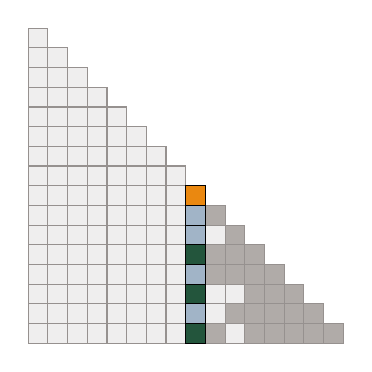
\begin{tikzpicture}[scale=4/16]
  \filldraw[draw=zeroborder, fill=zerocolor] (0, 0) rectangle (1, -1);
  \filldraw[draw=zeroborder, fill=zerocolor] (0, -1) rectangle (1, -2);
  \filldraw[draw=zeroborder, fill=zerocolor] (0, -2) rectangle (1, -3);
  \filldraw[draw=zeroborder, fill=zerocolor] (0, -3) rectangle (1, -4);
  \filldraw[draw=zeroborder, fill=zerocolor] (0, -4) rectangle (1, -5);
  \filldraw[draw=zeroborder, fill=zerocolor] (0, -5) rectangle (1, -6);
  \filldraw[draw=zeroborder, fill=zerocolor] (0, -6) rectangle (1, -7);
  \filldraw[draw=zeroborder, fill=zerocolor] (0, -7) rectangle (1, -8);
  \filldraw[draw=zeroborder, fill=zerocolor] (0, -8) rectangle (1, -9);
  \filldraw[draw=zeroborder, fill=zerocolor] (0, -9) rectangle (1, -10);
  \filldraw[draw=zeroborder, fill=zerocolor] (0, -10) rectangle (1, -11);
  \filldraw[draw=zeroborder, fill=zerocolor] (0, -11) rectangle (1, -12);
  \filldraw[draw=zeroborder, fill=zerocolor] (0, -12) rectangle (1, -13);
  \filldraw[draw=zeroborder, fill=zerocolor] (0, -13) rectangle (1, -14);
  \filldraw[draw=zeroborder, fill=zerocolor] (0, -14) rectangle (1, -15);
  \filldraw[draw=zeroborder, fill=zerocolor] (0, -15) rectangle (1, -16);
  \filldraw[draw=zeroborder, fill=zerocolor] (1, -1) rectangle (2, -2);
  \filldraw[draw=zeroborder, fill=zerocolor] (1, -2) rectangle (2, -3);
  \filldraw[draw=zeroborder, fill=zerocolor] (1, -3) rectangle (2, -4);
  \filldraw[draw=zeroborder, fill=zerocolor] (1, -4) rectangle (2, -5);
  \filldraw[draw=zeroborder, fill=zerocolor] (1, -5) rectangle (2, -6);
  \filldraw[draw=zeroborder, fill=zerocolor] (1, -6) rectangle (2, -7);
  \filldraw[draw=zeroborder, fill=zerocolor] (1, -7) rectangle (2, -8);
  \filldraw[draw=zeroborder, fill=zerocolor] (1, -8) rectangle (2, -9);
  \filldraw[draw=zeroborder, fill=zerocolor] (1, -9) rectangle (2, -10);
  \filldraw[draw=zeroborder, fill=zerocolor] (1, -10) rectangle (2, -11);
  \filldraw[draw=zeroborder, fill=zerocolor] (1, -11) rectangle (2, -12);
  \filldraw[draw=zeroborder, fill=zerocolor] (1, -12) rectangle (2, -13);
  \filldraw[draw=zeroborder, fill=zerocolor] (1, -13) rectangle (2, -14);
  \filldraw[draw=zeroborder, fill=zerocolor] (1, -14) rectangle (2, -15);
  \filldraw[draw=zeroborder, fill=zerocolor] (1, -15) rectangle (2, -16);
  \filldraw[draw=zeroborder, fill=zerocolor] (2, -2) rectangle (3, -3);
  \filldraw[draw=zeroborder, fill=zerocolor] (2, -3) rectangle (3, -4);
  \filldraw[draw=zeroborder, fill=zerocolor] (2, -4) rectangle (3, -5);
  \filldraw[draw=zeroborder, fill=zerocolor] (2, -5) rectangle (3, -6);
  \filldraw[draw=zeroborder, fill=zerocolor] (2, -6) rectangle (3, -7);
  \filldraw[draw=zeroborder, fill=zerocolor] (2, -7) rectangle (3, -8);
  \filldraw[draw=zeroborder, fill=zerocolor] (2, -8) rectangle (3, -9);
  \filldraw[draw=zeroborder, fill=zerocolor] (2, -9) rectangle (3, -10);
  \filldraw[draw=zeroborder, fill=zerocolor] (2, -10) rectangle (3, -11);
  \filldraw[draw=zeroborder, fill=zerocolor] (2, -11) rectangle (3, -12);
  \filldraw[draw=zeroborder, fill=zerocolor] (2, -12) rectangle (3, -13);
  \filldraw[draw=zeroborder, fill=zerocolor] (2, -13) rectangle (3, -14);
  \filldraw[draw=zeroborder, fill=zerocolor] (2, -14) rectangle (3, -15);
  \filldraw[draw=zeroborder, fill=zerocolor] (2, -15) rectangle (3, -16);
  \filldraw[draw=zeroborder, fill=zerocolor] (3, -3) rectangle (4, -4);
  \filldraw[draw=zeroborder, fill=zerocolor] (3, -4) rectangle (4, -5);
  \filldraw[draw=zeroborder, fill=zerocolor] (3, -5) rectangle (4, -6);
  \filldraw[draw=zeroborder, fill=zerocolor] (3, -6) rectangle (4, -7);
  \filldraw[draw=zeroborder, fill=zerocolor] (3, -7) rectangle (4, -8);
  \filldraw[draw=zeroborder, fill=zerocolor] (3, -8) rectangle (4, -9);
  \filldraw[draw=zeroborder, fill=zerocolor] (3, -9) rectangle (4, -10);
  \filldraw[draw=zeroborder, fill=zerocolor] (3, -10) rectangle (4, -11);
  \filldraw[draw=zeroborder, fill=zerocolor] (3, -11) rectangle (4, -12);
  \filldraw[draw=zeroborder, fill=zerocolor] (3, -12) rectangle (4, -13);
  \filldraw[draw=zeroborder, fill=zerocolor] (3, -13) rectangle (4, -14);
  \filldraw[draw=zeroborder, fill=zerocolor] (3, -14) rectangle (4, -15);
  \filldraw[draw=zeroborder, fill=zerocolor] (3, -15) rectangle (4, -16);
  \filldraw[draw=zeroborder, fill=zerocolor] (4, -4) rectangle (5, -5);
  \filldraw[draw=zeroborder, fill=zerocolor] (4, -5) rectangle (5, -6);
  \filldraw[draw=zeroborder, fill=zerocolor] (4, -6) rectangle (5, -7);
  \filldraw[draw=zeroborder, fill=zerocolor] (4, -7) rectangle (5, -8);
  \filldraw[draw=zeroborder, fill=zerocolor] (4, -8) rectangle (5, -9);
  \filldraw[draw=zeroborder, fill=zerocolor] (4, -9) rectangle (5, -10);
  \filldraw[draw=zeroborder, fill=zerocolor] (4, -10) rectangle (5, -11);
  \filldraw[draw=zeroborder, fill=zerocolor] (4, -11) rectangle (5, -12);
  \filldraw[draw=zeroborder, fill=zerocolor] (4, -12) rectangle (5, -13);
  \filldraw[draw=zeroborder, fill=zerocolor] (4, -13) rectangle (5, -14);
  \filldraw[draw=zeroborder, fill=zerocolor] (4, -14) rectangle (5, -15);
  \filldraw[draw=zeroborder, fill=zerocolor] (4, -15) rectangle (5, -16);
  \filldraw[draw=zeroborder, fill=zerocolor] (5, -5) rectangle (6, -6);
  \filldraw[draw=zeroborder, fill=zerocolor] (5, -6) rectangle (6, -7);
  \filldraw[draw=zeroborder, fill=zerocolor] (5, -7) rectangle (6, -8);
  \filldraw[draw=zeroborder, fill=zerocolor] (5, -8) rectangle (6, -9);
  \filldraw[draw=zeroborder, fill=zerocolor] (5, -9) rectangle (6, -10);
  \filldraw[draw=zeroborder, fill=zerocolor] (5, -10) rectangle (6, -11);
  \filldraw[draw=zeroborder, fill=zerocolor] (5, -11) rectangle (6, -12);
  \filldraw[draw=zeroborder, fill=zerocolor] (5, -12) rectangle (6, -13);
  \filldraw[draw=zeroborder, fill=zerocolor] (5, -13) rectangle (6, -14);
  \filldraw[draw=zeroborder, fill=zerocolor] (5, -14) rectangle (6, -15);
  \filldraw[draw=zeroborder, fill=zerocolor] (5, -15) rectangle (6, -16);
  \filldraw[draw=zeroborder, fill=zerocolor] (6, -6) rectangle (7, -7);
  \filldraw[draw=zeroborder, fill=zerocolor] (6, -7) rectangle (7, -8);
  \filldraw[draw=zeroborder, fill=zerocolor] (6, -8) rectangle (7, -9);
  \filldraw[draw=zeroborder, fill=zerocolor] (6, -9) rectangle (7, -10);
  \filldraw[draw=zeroborder, fill=zerocolor] (6, -10) rectangle (7, -11);
  \filldraw[draw=zeroborder, fill=zerocolor] (6, -11) rectangle (7, -12);
  \filldraw[draw=zeroborder, fill=zerocolor] (6, -12) rectangle (7, -13);
  \filldraw[draw=zeroborder, fill=zerocolor] (6, -13) rectangle (7, -14);
  \filldraw[draw=zeroborder, fill=zerocolor] (6, -14) rectangle (7, -15);
  \filldraw[draw=zeroborder, fill=zerocolor] (6, -15) rectangle (7, -16);
  \filldraw[draw=zeroborder, fill=zerocolor] (7, -7) rectangle (8, -8);
  \filldraw[draw=zeroborder, fill=zerocolor] (7, -8) rectangle (8, -9);
  \filldraw[draw=zeroborder, fill=zerocolor] (7, -9) rectangle (8, -10);
  \filldraw[draw=zeroborder, fill=zerocolor] (7, -10) rectangle (8, -11);
  \filldraw[draw=zeroborder, fill=zerocolor] (7, -11) rectangle (8, -12);
  \filldraw[draw=zeroborder, fill=zerocolor] (7, -12) rectangle (8, -13);
  \filldraw[draw=zeroborder, fill=zerocolor] (7, -13) rectangle (8, -14);
  \filldraw[draw=zeroborder, fill=zerocolor] (7, -14) rectangle (8, -15);
  \filldraw[draw=zeroborder, fill=zerocolor] (7, -15) rectangle (8, -16);
  \filldraw[draw=nnzborder, fill=nnzcolor] (9, -9) rectangle (10, -10);
  \filldraw[draw=zeroborder, fill=zerocolor] (9, -10) rectangle (10, -11);
  \filldraw[draw=nnzborder, fill=nnzcolor] (9, -11) rectangle (10, -12);
  \filldraw[draw=nnzborder, fill=nnzcolor] (9, -12) rectangle (10, -13);
  \filldraw[draw=zeroborder, fill=zerocolor] (9, -13) rectangle (10, -14);
  \filldraw[draw=zeroborder, fill=zerocolor] (9, -14) rectangle (10, -15);
  \filldraw[draw=nnzborder, fill=nnzcolor] (9, -15) rectangle (10, -16);
  \filldraw[draw=nnzborder, fill=nnzcolor] (10, -10) rectangle (11, -11);
  \filldraw[draw=nnzborder, fill=nnzcolor] (10, -11) rectangle (11, -12);
  \filldraw[draw=nnzborder, fill=nnzcolor] (10, -12) rectangle (11, -13);
  \filldraw[draw=zeroborder, fill=zerocolor] (10, -13) rectangle (11, -14);
  \filldraw[draw=nnzborder, fill=nnzcolor] (10, -14) rectangle (11, -15);
  \filldraw[draw=zeroborder, fill=zerocolor] (10, -15) rectangle (11, -16);
  \filldraw[draw=nnzborder, fill=nnzcolor] (11, -11) rectangle (12, -12);
  \filldraw[draw=nnzborder, fill=nnzcolor] (11, -12) rectangle (12, -13);
  \filldraw[draw=nnzborder, fill=nnzcolor] (11, -13) rectangle (12, -14);
  \filldraw[draw=nnzborder, fill=nnzcolor] (11, -14) rectangle (12, -15);
  \filldraw[draw=nnzborder, fill=nnzcolor] (11, -15) rectangle (12, -16);
  \filldraw[draw=nnzborder, fill=nnzcolor] (12, -12) rectangle (13, -13);
  \filldraw[draw=nnzborder, fill=nnzcolor] (12, -13) rectangle (13, -14);
  \filldraw[draw=nnzborder, fill=nnzcolor] (12, -14) rectangle (13, -15);
  \filldraw[draw=nnzborder, fill=nnzcolor] (12, -15) rectangle (13, -16);
  \filldraw[draw=nnzborder, fill=nnzcolor] (13, -13) rectangle (14, -14);
  \filldraw[draw=nnzborder, fill=nnzcolor] (13, -14) rectangle (14, -15);
  \filldraw[draw=nnzborder, fill=nnzcolor] (13, -15) rectangle (14, -16);
  \filldraw[draw=nnzborder, fill=nnzcolor] (14, -14) rectangle (15, -15);
  \filldraw[draw=nnzborder, fill=nnzcolor] (14, -15) rectangle (15, -16);
  \filldraw[draw=nnzborder, fill=nnzcolor] (15, -15) rectangle (16, -16);
  \filldraw[draw=colborder, fill=targetcolor] (8, -8) rectangle (9, -9);
  \filldraw[draw=colborder, fill=candcolor] (8, -9) rectangle (9, -10);
  \filldraw[draw=colborder, fill=candcolor] (8, -10) rectangle (9, -11);
  \filldraw[draw=colborder, fill=selcolor] (8, -11) rectangle (9, -12);
  \filldraw[draw=colborder, fill=candcolor] (8, -12) rectangle (9, -13);
  \filldraw[draw=colborder, fill=selcolor] (8, -13) rectangle (9, -14);
  \filldraw[draw=colborder, fill=candcolor] (8, -14) rectangle (9, -15);
  \filldraw[draw=colborder, fill=selcolor] (8, -15) rectangle (9, -16);
\end{tikzpicture}
%
    \qquad
    \input{figures/points_knn/selected_points_08.tex}
  \end{figure}
}
\only<9>{
  \begin{figure}
    \centering
    \input{figures/points_knn/cholesky_factor_09.tex}%
    \qquad
    \begin{tikzpicture}[baseline]
  \begin{axis}[
    % calculated from Cholesky factor, exactly 16 cm x 16 cm
    width={4cm},
    height={4cm},
    axis lines={none},
    % force axis box to have exactly the right dimensions, ignoring labels
    scale only axis=true,
  ]
  % consistent size bounding box
  \draw [white, line width=0] (-0.1, -0.1) -- (-0.1,  1.1);
  \draw [white, line width=0] ( 1.1, -0.1) -- ( 1.1,  1.1);
  \draw [white, line width=0] (-0.1, -0.1) -- (-1.1, -0.1);
  \draw [white, line width=0] (-0.1,  1.1) -- (-1.1,  1.1);
  \draw [seagreen!15, fill, radius=0.452634334564209] (0.29840122301687566, 0.3139860020343368) circle;
  \draw [seagreen, radius=0.452634334564209] (0.29840122301687566, 0.3139860020343368) circle;
  \draw [orange!25, fill, radius=0.2263171672821045] (0.29840122301687566, 0.3139860020343368) circle;
  \draw [orange, radius=0.2263171672821045] (0.29840122301687566, 0.3139860020343368) circle;
  \addplot [only marks, mark size=1, silver]    table
    {figures/points_knn/all_points.csv};
  \addplot [only marks, mark size=2, lightblue] table
    {figures/points_knn/candidates_09.csv};
  \addplot [only marks, mark size=4, seagreen]  table
    {figures/points_knn/selected_09.csv};
  \addplot [only marks, mark size=4, orange]    table
    {figures/points_knn/target_09.csv};
  \end{axis}
\end{tikzpicture}

  \end{figure}
}
\only<10>{
  \begin{figure}
    \centering
    \input{figures/points_knn/cholesky_factor_10.tex}%
    \qquad
    \input{figures/points_knn/selected_points_10.tex}
  \end{figure}
}
\only<11>{
  \begin{figure}
    \centering
    \input{figures/points_knn/cholesky_factor_11.tex}%
    \qquad
    \input{figures/points_knn/selected_points_11.tex}
  \end{figure}
}
\only<12>{
  \begin{figure}
    \centering
    \input{figures/points_knn/cholesky_factor_12.tex}%
    \qquad
    \begin{tikzpicture}[baseline]
  \begin{axis}[
    % calculated from Cholesky factor, exactly 16 cm x 16 cm
    width={4cm},
    height={4cm},
    axis lines={none},
    % force axis box to have exactly the right dimensions, ignoring labels
    scale only axis=true,
  ]
  % consistent size bounding box
  \draw [white, line width=0] (-0.1, -0.1) -- (-0.1,  1.1);
  \draw [white, line width=0] ( 1.1, -0.1) -- ( 1.1,  1.1);
  \draw [white, line width=0] (-0.1, -0.1) -- (-1.1, -0.1);
  \draw [white, line width=0] (-0.1,  1.1) -- (-1.1,  1.1);
  \draw [seagreen!15, fill, radius=0.3662240505218506] (0.6962159966701554, 0.2927207490124871) circle;
  \draw [seagreen, radius=0.3662240505218506] (0.6962159966701554, 0.2927207490124871) circle;
  \draw [orange!25, fill, radius=0.1831120252609253] (0.6962159966701554, 0.2927207490124871) circle;
  \draw [orange, radius=0.1831120252609253] (0.6962159966701554, 0.2927207490124871) circle;
  \addplot [only marks, mark size=1, silver]    table
    {figures/points_knn/all_points.csv};
  \addplot [only marks, mark size=2, lightblue] table
    {figures/points_knn/candidates_12.csv};
  \addplot [only marks, mark size=4, seagreen]  table
    {figures/points_knn/selected_12.csv};
  \addplot [only marks, mark size=4, orange]    table
    {figures/points_knn/target_12.csv};
  \end{axis}
\end{tikzpicture}

  \end{figure}
}
\only<13>{
  \begin{figure}
    \centering
    \input{figures/points_knn/cholesky_factor_13.tex}%
    \qquad
    \begin{tikzpicture}[baseline]
  \begin{axis}[
    % calculated from Cholesky factor, exactly 16 cm x 16 cm
    width={4cm},
    height={4cm},
    axis lines={none},
    % force axis box to have exactly the right dimensions, ignoring labels
    scale only axis=true,
  ]
  % consistent size bounding box
  \draw [white, line width=0] (-0.1, -0.1) -- (-0.1,  1.1);
  \draw [white, line width=0] ( 1.1, -0.1) -- ( 1.1,  1.1);
  \draw [white, line width=0] (-0.1, -0.1) -- (-1.1, -0.1);
  \draw [white, line width=0] (-0.1,  1.1) -- (-1.1,  1.1);
  \draw [seagreen!15, fill, radius=0.3178281784057617] (0.28420116374879145, 0.648547207079825) circle;
  \draw [seagreen, radius=0.3178281784057617] (0.28420116374879145, 0.648547207079825) circle;
  \draw [orange!25, fill, radius=0.15891408920288086] (0.28420116374879145, 0.648547207079825) circle;
  \draw [orange, radius=0.15891408920288086] (0.28420116374879145, 0.648547207079825) circle;
  \addplot [only marks, mark size=1, silver]    table
    {figures/points_knn/all_points.csv};
  \addplot [only marks, mark size=2, lightblue] table
    {figures/points_knn/candidates_13.csv};
  \addplot [only marks, mark size=4, seagreen]  table
    {figures/points_knn/selected_13.csv};
  \addplot [only marks, mark size=4, orange]    table
    {figures/points_knn/target_13.csv};
  \end{axis}
\end{tikzpicture}

  \end{figure}
}
\only<14>{
  \begin{figure}
    \centering
    \input{figures/points_knn/cholesky_factor_14.tex}%
    \qquad
    \begin{tikzpicture}[baseline]
  \begin{axis}[
    % calculated from Cholesky factor, exactly 16 cm x 16 cm
    width={4cm},
    height={4cm},
    axis lines={none},
    % force axis box to have exactly the right dimensions, ignoring labels
    scale only axis=true,
  ]
  % consistent size bounding box
  \draw [white, line width=0] (-0.1, -0.1) -- (-0.1,  1.1);
  \draw [white, line width=0] ( 1.1, -0.1) -- ( 1.1,  1.1);
  \draw [white, line width=0] (-0.1, -0.1) -- (-1.1, -0.1);
  \draw [white, line width=0] (-0.1,  1.1) -- (-1.1,  1.1);
  \addplot [only marks, mark size=1, silver]    table
    {figures/points_cknn/all_points.csv};
  \addplot [only marks, mark size=2, lightblue] table
    {figures/points_cknn/candidates.csv};
  \addplot [only marks, mark size=4, seagreen]  table
    {figures/points_cknn/selected_14.csv};
  \addplot [only marks, mark size=4, orange]    table
    {figures/points_cknn/target.csv};
  \end{axis}
\end{tikzpicture}

  \end{figure}
}
\only<15>{
  \begin{figure}
    \centering
    \input{figures/points_knn/cholesky_factor_15.tex}%
    \qquad
    \input{figures/points_knn/selected_points_15.tex}
  \end{figure}
}
\only<16>{
  \begin{figure}
    \centering
    \input{figures/points_knn/cholesky_factor_16.tex}%
    \qquad
    \input{figures/points_knn/selected_points_16.tex}
  \end{figure}
}
\end{frame}

\begin{frame}
\frametitle{Kullback-Leibler minimization}
\framesubtitle{}
\begin{wideitemize}
  \item<+-> Compute entries by minimizing Kullback-Leibler divergence
    \begin{align*}
      L \defeq \argmin_{\hat{L} \in \SpSet} \,
        \KL*{\N(\vec{0}, \CM)}
            {\N(\vec{0}, (\hat{L} \hat{L}^{\top})^{-1})}
    \end{align*}
  \item<+-> Efficient and embarrassingly parallel closed-form solution
    \begin{align*}
      L_{s_i, i} &= \frac{\CM_{s_i, s_i}^{-1} \vec{e}_1}
        {\sqrt{\vec{e}_1^{\top} \CM_{s_i, s_i}^{-1} \vec{e}_1}}
    \end{align*}
  \item<+-> Achieves state of the art \( \epsilon \)-accuracy in time
    complexity \( \BigO\left (N \log^{2d}\left (\frac{N}{\epsilon} \right
    ) \right ) \) with \( \BigO\left (N \log^{d}\left (\frac{N}{\epsilon}
    \right ) \right ) \) nonzero entries [\cite{schafer2021sparse}]
\end{wideitemize}
\end{frame}

\begin{frame}
\frametitle{Geometric dependence}
\framesubtitle{}

\begin{wideitemize}
  \item<+-> Screening effect motivated by geometric considerations
  \item<+-> Maximin ordering worse than
    random for spatial dimension \( \geq 4 \)
  \item<2-> Nearest neighbors unclear for paths
  \item<+-> Quick fix: correlation distance
    \begin{align*}
      \mathsf{dist}(p, q) &\defeq \sqrt{1 - \abs{\rho}} \\
      \rho(p, q) &\defeq \frac{k(p, q)}{\sqrt{k(p, p) k(q, q)}}
    \end{align*}
\end{wideitemize}
\end{frame}

\begin{frame}
\frametitle{Towards geometry-free Cholesky factors}
\framesubtitle{}

\begin{wideitemize}
  \item RPCholesky [\cite{chen2023randomly}] + random ordering
  \item RPCholesky + nearest neighbors + random candidate sets
  \item Conditional selection sparsity pattern [\cite{huan2023sparse}]
  \item Automatic interpolation between low rank/sparse
\end{wideitemize}
\end{frame}

\section{Conclusion}

\begin{frame}
\frametitle{Summary}
\framesubtitle{}

\begin{wideitemize}
  \item Non-ergodic earthquake models with Gaussian processes
  \item Efficient computation with sparse Cholesky factors
  \item Implemented in Julia, scale to HPC/supercomputers
  \item Project website and additional resources can be found at
    \begin{center}
      \url{https://kolesky.cgdct.moe}
    \end{center}
\end{wideitemize}
\end{frame}

\begin{frame}
\frametitle{}
\framesubtitle{}

% https://tex.stackexchange.com/questions/247826/beamer-full-vertical-centering
\begin{minipage}[c][0.99\textheight][c]{\linewidth}
  \centering
  {\huge \textcolor{lightblue}{Thank you!}} \\
\end{minipage}
\end{frame}

\begin{frame}[allowframebreaks]
\frametitle{References}
\framesubtitle{}

\printbibliography
\end{frame}

\begin{frame}
\frametitle{Kernels on paths}
\framesubtitle{}

\begin{wideitemize}
  \item Integral of a Mat{\'e}rn kernel \( k(\vec{x}, \vec{x}') \)
  \item If \( f \sim \GP(\vec{0}, k) \), then define \(
    \widetilde{f} = \int_0^1 f(\vec{x} + t(\vec{x}' - \vec{x})) \dd t \)
  \item Linear transformation of a GP is also a GP
  \item It has covariance
    \begin{align*}
      \widetilde{k}(\vec{x}, \vec{x}', \vec{y}, \vec{y}') &=
        \int_0^1 \int_0^1
          k(\vec{x} + t(\vec{x}' - \vec{x}), \vec{y} + s(\vec{y}' - \vec{y}))
        \dd t \dd s
    \end{align*}
    which creates ``paths'' in the 2-d input space.
\end{wideitemize}
\end{frame}

\end{document}
